\chapter{Zpracování dat}

Úvod ke kapitole.... % dopsat!!!!!

\section{Popis obdržených dat}

Všechna data poskytnutá společností jsou uložena v databázi, ke které je byl zhotoven omezený přístup pro účely získání dat pro analýzy shrinku produktů společnosti. Zároveň s možností přístupu jsem obdržela i tabulku, která stručně komentuje všechny tabulky v databázi a sloupce v jednotlivých tabulkách. Celkem se v databázi nachází 412 tabulek, z nichž je potřeba vybrat ty s relevantními daty pro úlohu shrinků.

Z důvodu ochrany dat nelze uvádět přesné názvy tabulek, nicméně pro lepší orientaci v textu, každé použité tabulce přiřadím název, který odpovídá obsaženým datům v tabulce.

\subsubsection{Produkty}

Základní číselník s údaji o produktech, se nachází v tabulce \texttt{produkt} se 27 sloupci. 
\begin{itemize}
    \item ID produktu a ID prodejní varianty, spolu tvoří primární klíč. 
    \item Krátký a dlouhý název produktu
    \item Expirace produktu ve dnech (hodnoty 0,999 a NULL označují neomezenou expiraci)
    \item Rozměry produktu a jeho hmotnost
    \item ID kategorie produktu v MS5 struktuře (pro lepší interpretaci, o jakou kategorii zboží se jedná, je výhodnější strukura 4BOX, kterou lze získat napojením )
\end{itemize}

Tabulka, která obsahuje 

\subsubsection{Tabulky transakcí}
V tabulce \texttt{transakce} se nachází údaje o všech provedených transakcích, a to jak skladové transakce, tak prodeje na prodejnách. V případě prodejen jsou údaje agregované podle prodejny, konkrétního produktu a dne transakce, tzn. v této tabulce nelze rozlišit konkrétní prodeje na jednotlivých pokladnách, ale pouze souhrn za jeden den. Tabulka obsahuje údaje za posledních dvanáct měsíců.

Tabulka transakcí obsahuje 21 sloupců, jako podstatné pro analýzu jsem vybrala následující sloupce:

\begin{itemize}
    \item ID transakce, jedinečné pro každou transakci
    \item Typ transakce
    \item ID produktu, kterého se transakce týká
    \item ID skladu (včetně prodejen)
    \item Datum transakce (tzv. business datum, pokud samotná transakce proběhne až po půlnoci uvedeného dne, tak se posílá s datem z předchozího dne, neboť do toho dne businessově náleží.)
    \item ID promoce 
    \item Motive\_type z hlediska hledání shrinku produktu se jedná o klíčový sloupec, neboť obsahuje označení jednotlivých typů shrinků.
    \item Množství produktu v dané transakci
    \item Hodnota transakce v nákladové ceně
    \item Hodnota transakce v prodejní ceně včetně DPH -- v případě prodejů se jedná o skutečnou cenu, u zbylých transakcích je uvedena odpovídající cena podle ceníku.
\end{itemize}

Tabulku, která obsahuje údaje o jednotlivých prodejích na prodejnách společnosti, jsem pro účely této práce nazvala \texttt{transakce\_prodeje}. Celkem obsahuje třináct sloupců, z nichž jsem vybrala následující:

\begin{itemize}
    \item ID transakce
    \item ID produktu, kterého se transakce týká
    \item ID prodejny
    \item Datum a čas transakce 
    \item ID promoce
    \item Množství produktu v dané transakci
    \item Hodnota transakce v prodejní ceně bez DPH
    \item Hodnota DPH dané transakce
\end{itemize}

\subsubsection{Tabulky ceníků}





\section{Statistické zpracování dat}



\subsection*{Sledované údaje}



\subsection*{Období jednoho měsíce}
\subsection*{Období jednoho roku}


Sledovala jsem tři různé veličiny, kterými lze hodnotit transakce - počet záznamů (tj. počet řádků) v tabulce \texttt{transakce}, celkové množství produktů a celková nákladová cena produktů. 

Z databáze jsem vybrala všechny transakce za rok 2022, u kterých byl evidován nějaký typ shrinku. Celkem se jednalo o %doplnit!!!
záznamů. Data jsem agregovala po jednotlivých měsících a pro každý měsíc vypočítala pomocí nástroje pivottables.


typ shrinku v závislosti na expiraci
typ shrinku v závislosti hlavní kategorii produktu
typ shrinku v závislosti na dni v měsíci
typ shrinku v závislosti na dni v týdnu

typ shrinku v závislosti na prodejně, neboli typu prodejny nebo v závislosti na centrálním skladu.
Závislost mezi prodejnami a typem produktu


\subsubsection*{Celkový přehled}

Nejprve jsem určila zastoupení jednotlivých shrinků během celého roku, a to bez uvažování závislosti na jiných faktorech. Poměr rozdělení lze vidět na obrázku \ref*{obr:rok:g:celkemD}.
Největší zastoupení, z pohledu všech tří sledovaných charakteristik, má shrink označující prošlé a zkažené zboží. Z pohledu počtu záznamů činí $70{,}24$ \% ze všech shrinků typu damage, což odpovídá 13 milionům řádkům záznamů. V případě množství neprodaných kusů produktů bylo v roce 2022 odepsáno 40 milionů kusů (tj. $65{,}67$  \%). Podle nejdůležitějšího ukazatele - nákladové ceny - tento shrink měl za následek ztrátu 635 milionů Kč (tj. $57{,}94$) \%.
Další damage shrinky, které mají zastoupení větší než 10  \% je shrink označující poškozené zboží a shrink s produkty, které byly odevzdány potravinové bance.
Zbylé shrinky mají v ročním pohledu malý počet výskytů a jejich výskyt bude analyzován v závislosti na dalších faktorech. 

\begin{figure}[hbtp!]
    \centering
    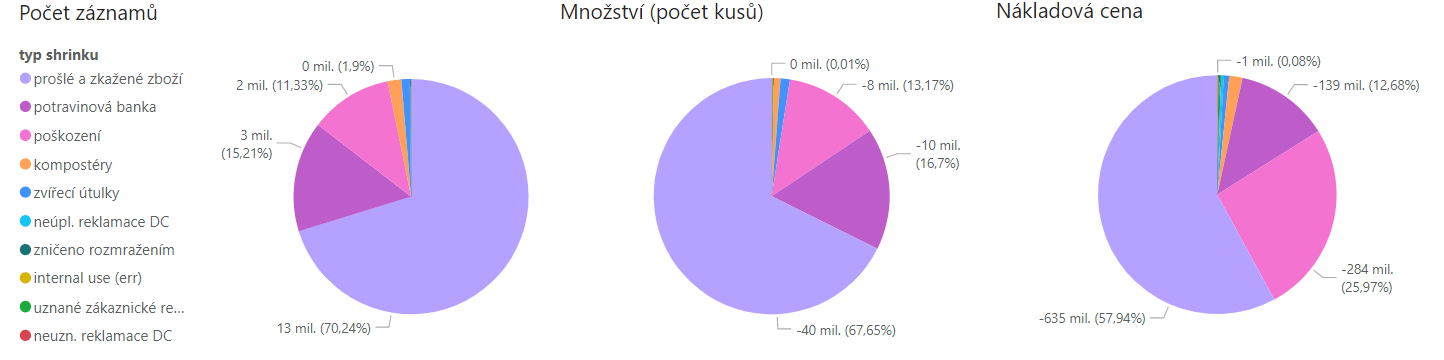
\includegraphics[width=\textwidth]{obrazky/grafy/Graf_celkem-D.png}
    \caption{Zastoupení shrinků typu damage v roce 2022.}
    \label{obr:rok:g:celkemD}
\end{figure}

\subsubsection*{Závislost typu shrinku na čase}

Porovnala jsem množství zaznamenaných shrinků v závislosti na dnech v týdnu, porovnání lze vidět na obr. \ref*{obr:rok:g:tydenD}. Jednotlivé typy jsou zastoupeny analogicky jako v souhrnném přehledu shrinků za jeden rok, tj. prošlé zboží, zboží zaslané do potravinové banky a poškozené zboží. Počty záznamů pro všechny dny jsou v rozmezí $1{,}6$ až $1{,}9$ milionů záznamů  za jeden rok. %!!! nebylo by lepsi tam dat prumer souctu za mesic za cely rok???

\begin{figure}[hbtp!]
    \centering
    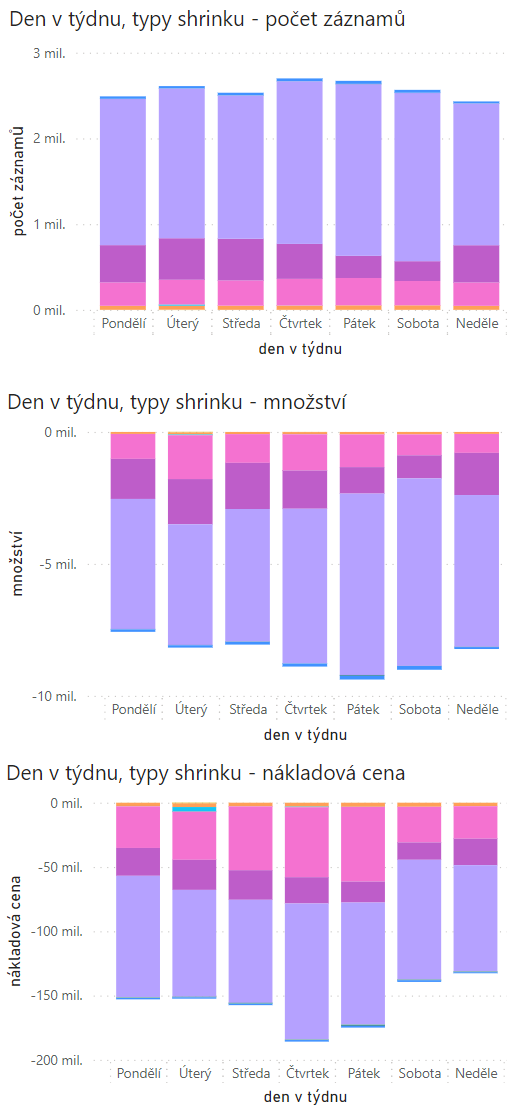
\includegraphics[width=0.5\textwidth]{obrazky/grafy/Grad_dny_tyden-D.png}
    \caption{Zastoupení shrinků typu damage v závislosti na dni v týdnu (údaje pro rok 2022).}
    \label{obr:rok:g:tydenD}
\end{figure}

\begin{figure}[hbtp!]
    \centering
    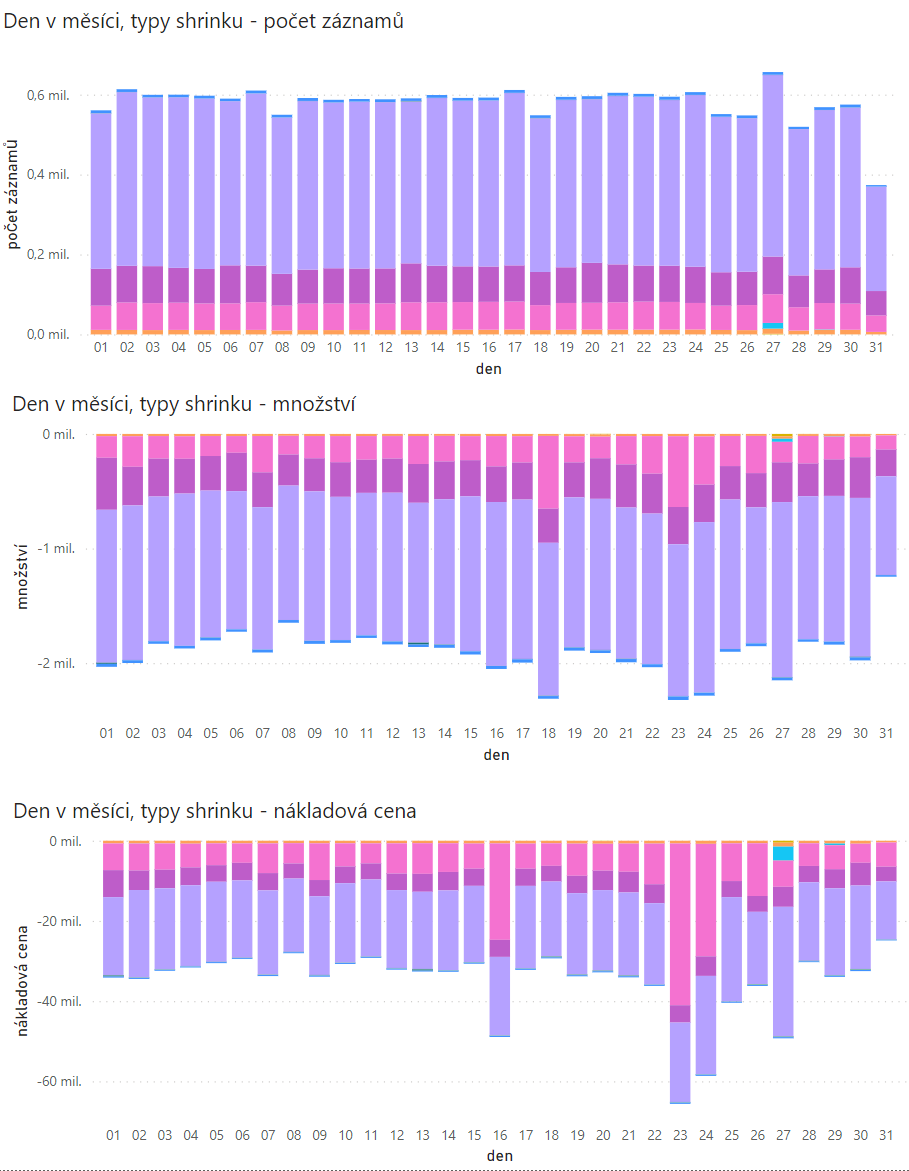
\includegraphics[width=\textwidth]{obrazky/grafy/Grad_dny_mesic-D.png}
    \caption{Zastoupení shrinků typu damage v závislosti na dni v měsíci (údaje pro rok 2022).}
    \label{obr:rok:g:mesicD}
\end{figure}

\subsubsection*{Závislost typu shrinku na hlavní kategorii zboží}

Kategorií, u které bylo evidováno nejvíce damage shrinků je kategorie produktů \emph{superfresh}. V rámci této kategorie je opět nejčastější příčinou odpisu zboží překročená doba expirace, u \emph{superfresh} produktů spíše viditelné zkažení zboží, neboť část \emph{superfresh} produktů nemá uvedenou dobu spotřeby. Druhý nejčastější shrink je shrink označující potravinovou banku. Zbylé shrinky jsou pro tuto kategorii již méně zastoupeny. Kategorie \emph{superfresh} má největší zastoupení většiny typů shrinků nad ostatními kategoriemi - přehled zastoupení jednotlivých shrinků odděleně je na obr. \ref{} %!!! udělat obrazek kde budou vedle sebe grafiký pro kazdy shrink


\subsubsection*{Závislost typu shrinku na typu prodejny}



